\documentclass[UTF8]{ctexart}

\usepackage{parskip}
    \setlength{\parindent}{0em}
    \setlength{\parskip}{1em}
\usepackage{geometry}
    \geometry{left=3.5cm,right=3.5cm,top=2cm,bottom=2cm}
\usepackage{amsmath, amssymb, amsthm, mathtools}
\usepackage{thmtools}
    \declaretheorem[numberwithin=section,shaded={rulecolor=cyan,rulewidth=2pt,bgcolor=white}]{definition}
    \declaretheorem[numberwithin=section,shaded={rulecolor=orange,rulewidth=2pt, bgcolor=white}]{theorem}
    \renewcommand\qedsymbol{$\blacksquare$}
    \newtheorem*{remark}{Remark}
    \newtheorem{proposition}{Proposition}[section]
\usepackage{tcolorbox}
    \newtcolorbox{conclusion}{colback=red!5!white,colframe=red!75!black}
\usepackage{caption} 	 % 标题
\usepackage{xcolor} 	 % 颜色
\usepackage{graphicx} 	 % 引用图片
\usepackage{float}
\usepackage{setspace} 	 % 行间距 \begin{spacing}{arg}
\usepackage{extarrows} 	 % 箭头宏包 \xLongrightarrow 
\usepackage{esvect} 	 % 向量箭头 \vv{}
\usepackage{siunitx} 	 % 国际单位 \si{unit} \SI{number}{unit} 
\usepackage{esint} 	 % 积分符号
\usepackage{mathrsfs}
\usepackage{hyperref}  % 超链接 用于使目录可点击跳转
    \hypersetup{
        colorlinks=true, %set true if you want colored links
        linktoc=all,     %set to all if you want both sections and subsections linked
        linkcolor=blue,  %choose some color if you want links to stand out
    }

% font
\newcommand{\ve}[1]{\boldsymbol{\mathbf{#1}}}
\newcommand{\unit}[1]{\boldsymbol{\mathbf{\hat{#1}}}}
\renewcommand{\r}{\mathrm}
\renewcommand{\cal}{\mathcal}
\newcommand{\scr}{\mathscr}
% common symbol
\newcommand{\E}{\mathrm e}
\renewcommand{\I}{\mathrm i}
\newcommand{\R}{\mathbb R}
\newcommand{\Z}{\mathbb Z}
\newcommand{\N}{\mathbb N}
\newcommand{\Q}{\mathbb Q}
\renewcommand{\C}{\mathbb C}
% differentiation
\def \DD #1.#2.#3 {\dfrac{d^{#1} #2}{d #3^{#1}}}
\def \PP #1.#2.#3 {\dfrac{\partial^{#1} #2}{\partial #3^{#1}}}
\def \dd #1.#2 {\dfrac{d #1}{d #2}}
\def \pp #1.#2 {\dfrac{\partial #1}{\partial #2}} 
\newcommand{\del}{\nabla}
% other
\newcommand{\transp}{^{\top}}
\DeclareMathOperator{\tr}{tr}
\DeclareMathOperator{\sgn}{sgn}

\pagestyle{empty}


\begin{document}
\tableofcontents

\newpage
\section{预备知识}
\subsection{点与向量}
一个点常见的表示方式为大写字母, 如 $ P $. 这种表示方式通常用于低维 ($ \R $, $ \R^2 $ 和 $ \R^3 $) 空间. 当涉及到高维空间 $ \R^n\, (n \geqslant 4) $ 时, 通常将点写作粗体, 即使用向量的表示方式, 如 $ \ve x = (x_1, x_2, \dots x_n) $. 为了和向量区分, 可能会见到 $ \ve x $ 表示点, $ \vec{\ve x} $ 或 $ \vec x $ 表示向量. 于此同时, 使用坐标表示时, 亦可能见到用圆括号 $ (x_1, x_2) $ 表示点, 尖括号表示向量 $ \langle x_1, x_2 \rangle $.

本文档约定下列表示方法:
\begin{itemize}
    \item 点和向量使用相同的表示方法, 不加区分, 如: $ \ve x $
    \item $ \R $, $ \R^2 $ 和 $ \R^3 $ 空间中的点可以使用大写斜体字母表示, 如: $ P $
    \item 点的坐标用圆括号, 如: $ (x, y, z) $; 如需要区分, 向量用尖括号, 如: $ \langle x_1, x_2, x_3 \rangle $
\end{itemize}

\paragraph{区分点和向量}
点和向量, 是有序 $ n $-元组的不同解释. 尤其是坐标表示, 除了使用括号不同, 似乎没有区别:\[ (x, y, z) \text{ 和 } \langle x, y, z \rangle \,.\]

并且用向量表示点的方式也很常见, 如位置向量. 但其实\textbf{在欧几里得空间中, 区分点和向量是有好处的,} 尽管在大多数地方将点解释为位置向量或反之都不会产生影响.

\paragraph{空间与点} 
在低于 $ 4 $ 维的空间中, 可视化一个点是十分容易的. 但高维空间, 及其中的点都不容易可视化. 此时将一个点看作一种\textbf{状态}可以便于理解. 设想一个人的六门成绩: 语数外物化生; 每一门的取值, 即 $ [0..100] $ \footnote{$ [a..b] $ 表示整数区间, 即 $ [a, b] $ 区间中所有的整数} 记作一个集合 $ S $. 则六门科目的成绩就可以形成 $ 6^{101} $ 种情况(状态), 构成一个空间 $ S^6 $ (笛卡尔积相关内容). 里面每一种状态, 就是这个``成绩空间''中的一个点. 如: $ (90, 95, 95, 90, 80, 85) $, 就是一种成绩的状态. 通过类比, $ \R^n $ 空间, 以及此空间中的点就很好理解了. 此外, 从编程的角度, 空间可以看成一个类, 点可以看成空间的实例化 :)

\paragraph{向量} 
向量被定义为既有大小又有方向的量, 这个定义没有问题. 但在数学上, 向量还可以被解释为从一个点到另一个点的坐标变化. 还是那上面的成绩空间举例, 从第一次的成绩 $ \ve s_1 = (90, 95, 95, 90, 80, 85) $ 到第二次 $ \ve s_2 = (91, 95, 95, 90, 78, 83) $, 可以看出: 语文涨了 1 分, 化学和生物跌了 2 分. 所以很自然地 $ \ve s_2 - \ve s_1 = \langle 1, 0, 0, 0, -2, -2 \rangle $, 这样得到的就是向量.

\begin{conclusion}
    \textbf{点作为空间中的位置, 表示了一种状态. 向量作为点位置的变化, 表示了状态的变化. 将 $ (x_1, x_2, \dots, x_n) $ 同时看成点和(位置)向量或是将其区分开一般都可以接受.}
\end{conclusion}


\paragraph{点和向量的运算}
根据上面的参数, 不难得到:
\[ \text{点} - \text{点} = \text{向量} \,,\]

准确地说: 终点 $ - $ 起点 $ = $ 起点到终点的向量.
\[ \text{点} + \text{向量} = \text{点} \,,\]
\[ \text{向量} \pm \text{向量} = \text{向量} \,.\]

\subsection{集合}
\begin{definition}[\text{可数集合}]
    一个集合可数, 如果这个集合可以计数, 即每个元素可以对应一个自然数. 换句话说, 这个集合中的元素可以逐个列出, 故也称可列集.
\end{definition}

可数分为有限可数(至多可数)和无穷可数. 如 $ {a, b, c, d} $ 是一个有限可数集; $ \Z $ 是一个无穷可数集, 因为 $ \Z $ 中的元素可以逐个列出 $ 0, \pm 1, \pm 2, \dots $

\begin{definition}[\text{可数并集}]
    可数个集合的并集称为可数并集, 比如对于一系列集合 $ A_1, A_2, \dots $, $ A_1 \cup A_2 \cup \cdots \cup A_n $, 或有限个或可数无穷个集合的并集. 记作 $\displaystyle \bigcup_{i = 1}^n A_i $ 或 $\displaystyle \bigcup_{i\in\N} A_i $.
\end{definition}

\begin{theorem}[\text{可数集并集}]
    可数个可数集的并集, 即可数集的可数并集, 仍然是可数集.
\end{theorem}

可通过对角线法说明. 注意, 此处的可数, 包括有限可数和无穷可数.

\subsubsection{集合的开闭}
\begin{definition}[\text{开球}]
    $ \ve x \in \R^n $, $ B_r (\ve x) \coloneqq \{ \ve y \in \R^n \colon |\ve x - \ve y| < r \} $ 称为 $ \R^n $ 中的开球.
\end{definition}

欧氏空间中可以定义距离 $ d(\ve x, \ve y) = \sqrt{x_1^2 + x_2^2 + \cdots + x_n^2} $, 和 $ |\ve x - \ve y| $ 等价.

在 $ \R^3 $ 及更高维的空间中 $ B_r(\ve x) $ 称之为球; 特殊到 $ \R^2 $ 平面上, 这个开球就拍扁成开圆盘; 而在实数轴 $ \R $ 上, 开球就表现为以 $ x $ 为中心的开区间.

\begin{definition}[\text{开集}]
    $ \R^n $ 中有集合 $ U $. 若 $ \forall \ve x \in U $, $ \exists r > 0 $, 使得 $ B_r (\ve x) \subset U $, 则称 $ U $ 为 $ \R^n $ 中的开集.
\end{definition}

一个集合的内部点沿所有方向抖动一下, 通过控制抖动的距离, 是可以控制点始终在集合内的. 而边界点不行, 无论抖动多微小, 总会出现一些方向, 点离开集合. 所以开集定义的实质就是判断是否所有点都存在邻域包含在集合中.

\begin{figure}[H]
    \centering
    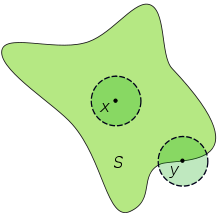
\includegraphics[width = 0.3\linewidth]{./images/set1.png}
\end{figure}


集合并非是``非开即闭'': 开集不包含任何边界; 闭集包含所有边界; 而包含部分边界的集合, 既不是开集也不是闭集. 同时要注意: 孤点也是边界.

\begin{definition}[\text{闭集}]
    对于 $ \R^n $ 中的集合 $ C $, 若其补集 $ \R^n \setminus C $ 是开集, 则 $ C $ 是闭集.
\end{definition}

关于区间: $ (a, b) $ 毫无疑问为开区间. $ (a, +\infty) $ 也是开区间. 而按照定义 $ [a, +\infty) $ 的补集为 $ (-\infty, a) $, 为开区间, 所以 $ [a, +\infty) $ 为闭区间.

\paragraph{例}
$ (1, 3) $, $ (1, 3) \cup (4, 5) $ 是开区间

$ [1, 3] $, $ [1, 3] \cup \{4\} $ 是闭区间

$ [1, 3) $, $ (1, 3) \cup \{4\} $ 既不是开区间也不是闭区间
\vskip 1em

\begin{proposition}
    两个开集的笛卡尔积也是开集.
\end{proposition}


\subsubsection{上确界和下确界}
\begin{definition}[\text{有界}]
    $ \R^n $ 中的 $ X $ 有界, 如果能够找到一个有限的 $ r $, 使得 $ X \subset B_r(0) $.
\end{definition}

\begin{definition}[\text{上界和下界}]
    对于集合 $ S \subset \R $, $ \exists M \in \R $, 使得 $ \forall s \in S $, $ s \leqslant M $, 则称 $ M $ 为 $ S $ 的\textbf{一个}上界. 同理若 $ \exists m \in \R $, 使得 $ \forall s \in S $, $ s \geqslant m $, 则称 $ m $ 为 $ S $ 的\textbf{一个}下界.
\end{definition}

注意集合内的任意元素不大于上界, 不小于下界, 但可以取等于. 也就是说, 上下界可以集合内的某个元素, 也可以不在这个集合中.

上界和下界是不唯一的. 但存在最小上界和最大下界, 即上确界和下确界. 集合 $ S $ 的上确界和下确界分别记为 $ \sup S $ 和 $ \inf S $.

下面以集合 $ S $ 举例, 设 $ S $ 的上界集合为 $ U $, 则最小上界 $ \beta $ 必然包含两个方面:
\begin{enumerate}
    \item $ \beta $ 是上界: $ \forall s \in S $, $ s \leqslant \beta $
    \item $ \beta $ 再小一点就不再是上界(即: 最小上界): $ \forall \epsilon > 0 $, $ \exists s \in S $, $ s > \beta - \epsilon $
\end{enumerate}

$ \beta - \epsilon $ 表示如果 $ \beta $ 再减小一点; 此时 $ \beta - \epsilon $ 就不再是上界, 意味着 $ S $ 中能够找到比 $ \beta - \epsilon $ 大的元素 $ s > \beta - \epsilon $.

\paragraph{例}
$ \sup\{x\in \mathbb {R} \mid 0<x<1\}=\sup\{x\in \mathbb {R} \mid 0\leq x\leq 1\} = 1 $

$ \inf\{1,2,3,\dots \}=1 $


\begin{theorem}[\text{确界存在定理}] 
    非空有上/下界的数集必有上/下确界.
\end{theorem}

\subsubsection{最大/最小值}
\begin{definition}
    若 $ \exists x \in S $, $ x = \sup S $, 则称 $ x $ 为 $ S $ 的最大值. 同理若 $ x = \inf S $, 则称 $ x $ 为 $ S $ 的最小值.
\end{definition}

前面提到, 上确界可以是集合的元素, 也可以不是. 当上确界是集合的元素时, 这个元素是集合的最大元素. 最小元素同理.
\paragraph{例}
$ \{ x \in \R \mid 0 < x < 1 \} $ 没有最大值, 但存在上确界为 1.

$ \{ x \in \R \mid 0 \leqslant x \leqslant 1 \} $ 有最大值 $ 1 $, 上确界 $ 1 $.

\subsection{序列, 函数与极限}
点序列 $ \ve a_1, \ve a_2, \ve a_3, \dots $ 记作 $ (\ve a_m) $ 或 $ \{ \ve a_m \} $.

从最初序列通过去除某些元素但不破坏余下元素的相对位置而形成的新序列, 称为原序列的子序列. 对于序列 $ a_1, a_2, \dots $, 其子序列可以表示为 $ a_{i(1)}, a_{i(2)}, \dots $. 

\begin{definition}[\text{$ \epsilon $-$ M $ 定义}]
    $ \R^n $ 中的点列 $ (\ve a_m) $ 收敛到 $ \ve a \in \R^n $, 如果 $ \forall \epsilon > 0 $, $ \exists M > 0 $, 使得当 $ m > M $ 时, $ |\ve a_m - \ve a| < \epsilon $. 记为 $\displaystyle \lim_{m \to \infty} \ve a_m = \ve a $, 或 $ \ve a_m \to \ve a\ (m \to \infty) $.
\end{definition}

换句话说: 无论 $ \epsilon $ 有多小, 总能找到一个界限 $ M $, 满足 $ M $ 之后的所有点 $ \ve a_m $ 和 $ \ve a $ 的距离都小于给定的 $ \epsilon $. 

\begin{proposition}
    $ \R^n $ 中的序列 $ (\ve a_m) = \ve a_1, \ve a_2, \dots $ 收敛于 $ \ve a $ 当且仅当序列的每一个分量收敛. 即对每一个 $ 1 \leqslant j \leqslant n $, 分量构成的序列 $ (a_m)_j $ 收敛于 $ a_j $. 其中 $ a_j $ 为 $ \ve a $ 的第 $ j $ 个分量.
\end{proposition}

\begin{definition}[\text{$ \epsilon $-$ \delta $ 定义}]
    如果 $ \forall \epsilon > 0 $, $ \exists \delta > 0 $, 使得 $ 0 < |\ve x - \ve x_0| < \delta $ 时, $ |f(\ve x) - f(\ve x_0) | < \epsilon $; 则称函数 $ f(\ve x) $ 有极限 $ f(\ve x_0) $. 记为 $ \displaystyle \lim_{\ve x \to \ve x_0} f(\ve x) = f(\ve x_0) $.
\end{definition}

按照定义, 极限为无穷也是极限不存在的一种情况.

引入邻域的定义 $ U(a, \delta) \coloneqq \{ x \colon |x - a| < \delta \} $, 即: 以 $ a $ 为中心, 半径为 $ \delta $ 的区间. 同理可以定义去心邻域 $ U_0(a, \delta) \coloneqq \{ x \colon 0 < |x - a| < \delta \} $, 即邻域 $ U(a, \delta) $ 去掉 $ a $ 点. 拓展到 $ \R^n $ 中, 则就回到最开始的开球定义: $ U(a, \delta) $ 可类比 $ B_\delta(a) $.

所以以一元函数为例, $ \epsilon $-$ \delta $ 定义中的条件可以重新阐述为: $ \forall \epsilon > 0 $, $ \exists \delta > 0 $, 使得当 $ x $ 在 $ U_0(x, \delta) $ 邻域里时, $ f(x) $ 和 $ f(x_0) $ 的距离小于 $ \epsilon $.
\vskip 1em

\begin{proposition}[$ \epsilon $-$ \delta $ 定义拓展]
    当 $ \epsilon \to 0 $ 时 $ u(\epsilon) \to 0 $, 则可用 $ u(\epsilon) $ 替换原定义中的 $ \epsilon $. 
\end{proposition}

$ \displaystyle \lim_{x \to 0} f(x) = 0 $, 此时的 $ f(x) $ 称为无穷小量. 所以上面的 $ u(\epsilon) $ 就是一个无穷小量.


\subsection{四大定理}
\subsubsection{紧致集}
\begin{definition}[\text{紧致集}]
    集合 $ C \subset \R^n $ 是闭集且有界, 则称其为紧致集.
\end{definition}

\begin{theorem}[\text{紧致集中的收敛子列}]
    若紧致集 $ C \subset \R^n $ 包含序列 $ \ve x_1, \ve x_2, \dots $, 则该序列拥有收敛子列 $ \ve x_{i(1)}, \ve x_{i(2)}, \dots $, 且其极限在 $ C $ 中.
\end{theorem}

即: 紧致集中的序列有收敛子列.

注意: 显然子集不能取等 $ C \subseteq \R^n $. $ \R^n $ 无界开区间.

\subsubsection{紧致集上的函数}
数列可以看成自然数定义域上的函数. 数列和函数也有有界, 上/下界, 上/下确界的概念, 且与集合类似. 同理可以定义函数的最值.

\begin{theorem}[\text{紧致集上的函数最值}]
    紧致集 $ C \subset \R^n $ 上的函数 $ f : C \to \R $ 连续. 则存在点 $ \ve a \in C $ 使得对 $ \forall \ve x \in C $ 都有 $ f(\ve a) \geqslant f(\ve x) $, 即最大值. 同理存在 $ \ve b \in C $ 使得 $ \forall \ve x \in C $ 都有 $ f(\ve b) \leqslant f(\ve x) $, 即最小值.
\end{theorem}

一句话概括, 紧致集上的连续函数有最值.

\subsubsection{中值定理}
\begin{theorem}[\text{中值定理}]
    $ f $ 是定义在 $ [a, b] $ 上的函数, $ f \in C^0[a, b] $, $ f \in C^1(a, b) $, 则 $ \exists c \in (a, b) $, 使得 \[ f'(c) = \dfrac{f(b) - f(a)}{b - a} \,.\]
\end{theorem}

$ f \in C^0 [a, b] $ 表示 $ f $ 在 $ [a, b] $ 上连续; $ f \in C^1 (a, b) $ 表示 $ f $ 在 $ (a, b) $ 上可导.

\subsubsection{代数基本定理}
\begin{theorem}[\text{代数基本定理}]
    $ n $ 次复系数多项式 \[ p(z) = a_n z^n + a_{n-1} z^{n-1} + \cdots + a_1 z + a_0 \ (a_n \neq 0) \] 必然有 $ n $ 个根 \rm{(}重根视为多个根\rm{)}. 且总能写成下面的形式: \[ a_n (z - z_1)(z - z_2) \cdots (z - z_n) \,,\] 其中, $ z_1, z_2, \dots, z_n $ 为 $ p(z) $ 的 $ n $ 个根.
\end{theorem}

\section{微分学}
\subsection{导数与偏导数}
\begin{definition}[\text{导数}]
    对一元函数 $ f: U \subseteq \R \to \R $, $ a $ 点处的导数定义为:\[ f'(a) = \lim_{h \to 0} \dfrac{f(a+h) - f(a)}{h} \,.\] 若该极限存在, 就称 $ f $ 在 $ a $ 处可导, 导数为 $ f'(x) $.
\end{definition}

亦等价于 \[ f'(a) = \lim_{x \to a} \dfrac{f(x) - f(a)}{x - a} \,.\]

\begin{remark}
    写成 $ f: U \subseteq \R \to \R $ 而非 $ f: \R \to \R $ 是必要的. 因为并非所有函数的定义域都是 $ \R $, 如 $ \ln x $, $ x^{-1} $ 等.
\end{remark}

\begin{definition}[\text{偏导数}]
    $ f: U \subseteq \R^n \to \R $ 的偏导数定义为: \[ \left. \pp {f(\ve x)}.{x_i} \right|_{\ve x = \ve a} = \lim_{h \to 0} \dfrac{f(a_1, \dots, a_i + h, \dots, a_n) - f(a_1, \dots, a_i, \dots, a_n)}{h} \,.\] 若该极限存在, 就称 $ f $ 在 $ \ve a $ 处存在偏导. 若 $ f $ 的 $ n $ 个偏导都存在, 则称 $ f $ 可导.
\end{definition}

偏导数描述了 $ f(\ve x) $ 在 $ x_i $ 方向上的导数(变化率). 偏导数可以看成一元函数导数的推广, 导数可以看成偏导数的特例.
\vskip 0.5em

\begin{remark}
    \begin{spacing}{1.6}
        偏导数的记号非常多, 如: $ \pp {f(x, y)}.{x} $, $ \pp {}.{x} f(x, y) $, $ \pp {f}.{x} (x_0, y_0) $, $ f_x $, $ \partial_x f $, $ \partial_1 f $, $ D_1 f $ 等. 其中的 $ x $ 均表示``对 $ x $ 的偏导'', $ 1 $ 表示 ``对第 $ 1 $ 个变量的偏导''.   
    \end{spacing}
\end{remark}

\begin{remark}
    \begin{spacing}{1.6}
        $ \pp {f(x, y)}.{x} $ 的记号可能带来歧义. 要区分开偏导函数和该函数在某一点处的值. $ \pp {f}.{x} $, $ \pp {f(x, y)}.{x} $, $ \pp {}.{x} f(x, y) $, $ f_x $, $ \partial_x f $ 等表示对 $ f(x, y) $ 的 $ x $ 变量求偏导. $ \left. \pp {f}.{x} \right|_{(x_0, y_0)} $, $ \pp {f}.{x} (x_0, y_0) $, $ f_x (x_0, y_0) $, $ \partial_x f(x_0, y_0) $ 等表示 $ (x_0, y_0) $ 处的偏导. 更加严谨的写法, 会将 $ \partial_x f(x_0, y_0) $ 和 $ D_1 f(x_0, y_0) $ 理解为对 $ f(x_0, y_0) $ 求导, 而把 $ (\partial_x f)(x_0, y_0) $ 和 $ (D_1 f)(x_0, y_0) $ 理解为 $ (x_0, y_0) $ 处的导数.
    \end{spacing}
\end{remark}

\begin{remark}
    \begin{spacing}{1.6}
        当一些自变量相关, 有时候必须明确哪些变量被视为常量, 可以使用下面的记号. 如: $ \left( \pp {f}.{x} \right)_{\! y, z} $, 表示对 $ x $ 求偏导, $ y $, $ z $ 视作常数. 气压函数自变量有体积, 温度, 物质的量, $ \pp {P}.{V} $ 表示气压对气体体积求导, 但改变了体积, 其它相关变量就会改变. 此时这个记号就出现了歧义. 所以如果保持温度不变是必要的, 就应该明确写出 $ \left( \pp {P}.{V} \right)_{\! T} $, 表示控制温度 $ T $ 为常量, 改变体积 $ V $. 同理可以有 $ \left( \pp {P}.{V} \right)_{\! n} $ 表示控制物质的量 $ n $, 改变体积.
    \end{spacing}
\end{remark}

\begin{definition}[\text{向量函数的偏导数}]
    $ \ve F: U \subseteq \R^n \to \R^m $, $ m > 1 $ 的导数定义如下: \[ \pp {\ve F}.{x_i} = \lim_{h \to 0} \dfrac{\ve F(x_1, \dots, x_i + h, \dots, x_n) - \ve F(x_1, \dots, x_i, \dots, x_n)}{h} \] 可以得到: \[ \pp {\ve F}.{x_i} = \left\langle \pp {F_1}.{x_i}, \pp {F_2}.{x_i}, \dots, \pp {F_m}.{x_i} \right\rangle \,.\]
\end{definition}

也即: 对向量求导, 就是对向量的各分量求导. 换种形式:
\[ D_i \ve F = \left\langle D_i F_1, D_i F_2, \dots, D_i F_m \right\rangle = \begin{bmatrix}
    D_i F_1 \\ D_i F_2 \\ \vdots \\ D_i F_m
\end{bmatrix} \,.\]

对多个变量同时求导, 可以将结果放到一个矩阵当中, 称为雅可比矩阵.

\begin{definition}[\text{雅可比矩阵}]
    $ \ve x \in \R^n $, $ \ve y \in \R^m $. 则 $ \ve y $ 对 $ \ve x $ 求导可以定义为一个 $ m \times n $ 雅可比矩阵: 
    \[ \pp {\ve y}.{\ve x} = 
        \begin{bmatrix}
            \pp {y_1}.{x_1} & \pp {y_1}.{x_2} & \cdots & \pp {y_1}.{x_n} \\
            \pp {y_2}.{x_1} & \pp {y_2}.{x_2} & \cdots & \pp {y_2}.{x_n} \\
            \vdots & \vdots & \ddots & \vdots  \\
            \pp {y_m}.{x_1} & \pp {y_m}.{x_2} & \cdots & \pp {y_m}.{x_n}
        \end{bmatrix}
    \] 
    也就是说, 雅可比矩阵 $ \left[ \pp {\ve y}.{\ve x} \right]_{m \times n} $ 的 $ i $ 行 $ j $ 列元素为:
    \[ \left[ \pp {\ve y}.{\ve x} \right]_{ij} = \pp {y_i}.{x_j} \,.\]
\end{definition}
\vskip 1em 

从左到右, 每一列是对变量分别求导; 从上到下, 每一行是对函数分量分别求导. 比如对 $ \ve f: \R^n \to \R^m $: 
\[ \pp {\ve f}.{\ve x} = \begin{bmatrix}
    D_1 \ve f & D_2 \ve f & \cdots & D_n \ve f \\
\end{bmatrix} \,.\]

随后就可以对 $ \ve f $ 求偏导, 即对各分量求导, $ n \times 1 $ 行矩阵就展开为一个 $ m \times n $ 矩阵.
\vskip 1em 

\begin{remark}
    $ \R^n \to \R^m $ 映射的雅可比矩阵也是 $ \R^n \to \R^m $, 大小为 $ m \times n $ \rm{(} $ m \to n $ 映射对应 $ n \times m $ 矩阵\rm{)}. $ m \times n $ 的矩阵作用在 $ n $ 维向量上, 得到 $ m $ 维向量, 即 $ m\times 1 $ 矩阵.
\end{remark}
\vskip 1em 

\begin{remark}
    雅可比矩阵和偏导的区别在于, 偏导只对一个变量求导, 其它变量视作常量; 而雅可比矩阵则是对考虑所有变量的变化, 类似于对所有变量同时求导, 所以是矩阵形式, 矩阵里面有各个偏导的信息.
\end{remark}

雅可比函数的重要性在于, 如果函数 $ \ve f: \R^n \to \R^m $ 可微, 点 $ \ve x $ 处的雅可比矩阵即为该函数在该点的最佳线性逼近, 也代表着雅可比矩阵是单变量实函数的微分在向量值多变量函数中的推广:
\[ \Delta \ve f = \ve f(\ve x + \ve h) - \ve f(\ve x) = \pp {\ve f}.{\ve h} \ve h + o(\|\ve h\|) \,;\]
\[ \Delta f = f(x + h) - f(x) = f'(x) h + o(h) \,.\]

$ f'(x) h $ 是函数值变化 $ \Delta f $ 的最佳线性近似; 同理 $ \pp {\ve f}.{\ve h} \ve h $ 也是向量函数变化量 $ \Delta \ve f $ 的最佳近似. 所谓最佳近似, 意味着 $ h \to 0 $ 时, $ f'(x) h \to \Delta f $. 所以雅可比矩阵也被称为 $ \ve f $ 在 $ \ve x $ 处的微分或导数. 也能看到下面的记号: $ D\ve f $, $ \ve J_{\ve f} $, $ D \ve f(\ve x) $.

\paragraph{例}
对于 $ \ve f(\ve x) = \ve f(x, y) = \left\langle xy, x + 2y, x^2 \sin y \right\rangle $:
\[ D\ve f = \ve J_{\ve f} = \begin{bmatrix}
    y & x \\
    1 & 2 \\
    2 x \sin y & x^2 \cos y
\end{bmatrix} \,,\]

对于点 $ \ve a = (2, \pi) $
\[ 
    D\ve f(\ve a) =  \begin{bmatrix}
        \pi & 2 \\
        1 & 2 \\
        0 & -4
    \end{bmatrix}\,.   
\]

考虑 $ \ve a $ 处的变量 $ \ve h = \langle h_1, h_2 \rangle $:
\[ \Delta \ve f = \ve f (\ve a + \ve h) - \ve f (\ve a) =  \]



总结一下:
\begin{table}[H]
    \centering
    \begin{tabular}{c|c|c|c}
    \hline
    函数名    & 映射 & (偏)导数 & 雅可比矩阵 \\ \hline
    一元标量函数 &  $ f: \R \to \R $  &   $ \dfrac{df}{dx} $   &  $ \big[ D f \big]_{1 \times 1} $     \\ \hline
    多元标量函数 &  $ f: \R^n \to \R $  &   $ \pp {f}.{x_i} $   &   $ \big[ D f \big]_{1 \times n} $    \\ \hline
    一元向量函数 &  $ \ve f: \R \to \R^m $  &   $ \pp {\ve f}.{x} $   &  $ \big[ D \ve f \big]_{m \times 1} $     \\ \hline
    多元向量函数 &  $ \ve f: \R^n \to \R^m $  &  $ \pp {\ve f}.{x_i} $    &   $ \big[ D \ve f \big]_{m \times n} $    \\ \hline
    \end{tabular}
\end{table}


\subsection{连续, 可导及可微}
对于一元标量函数, 可微和可导完全等价. 此时对于一个点, 可导(微)可以推出连续, 而连续不能推导出可(导)微.

而对于其它的函数, 可微和可导不同. 可微本质上是某一点处的局部线性近似, 而可导是一点处各个变量方向的变化率. 可微要求各个方向导数存在, 而可导只是有限个变量方向的偏导存在. 可见, 在非一元标量函数中, 可微要比可导强得多, 而可导又强于连续.

\begin{figure}[H]
    \centering
    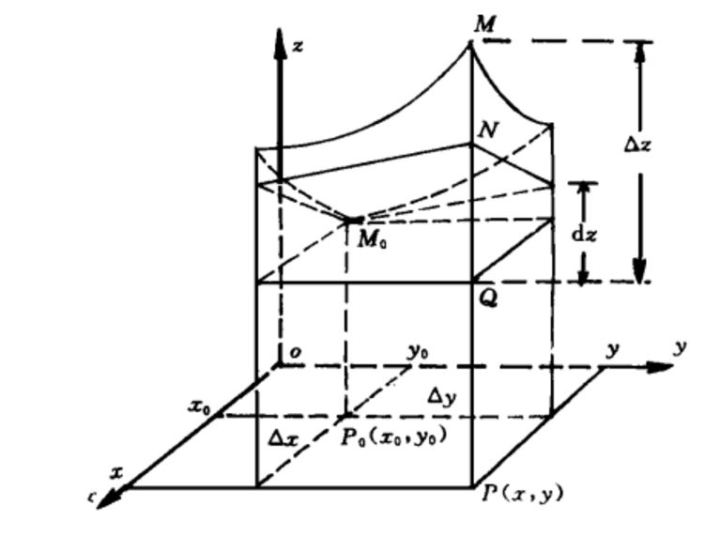
\includegraphics[width = 0.4\linewidth]{./images/diff.jpg}
    \caption{$ f:\R^2 \to \R $ 例图}
\end{figure}


\begin{figure}[H]
    \centering
    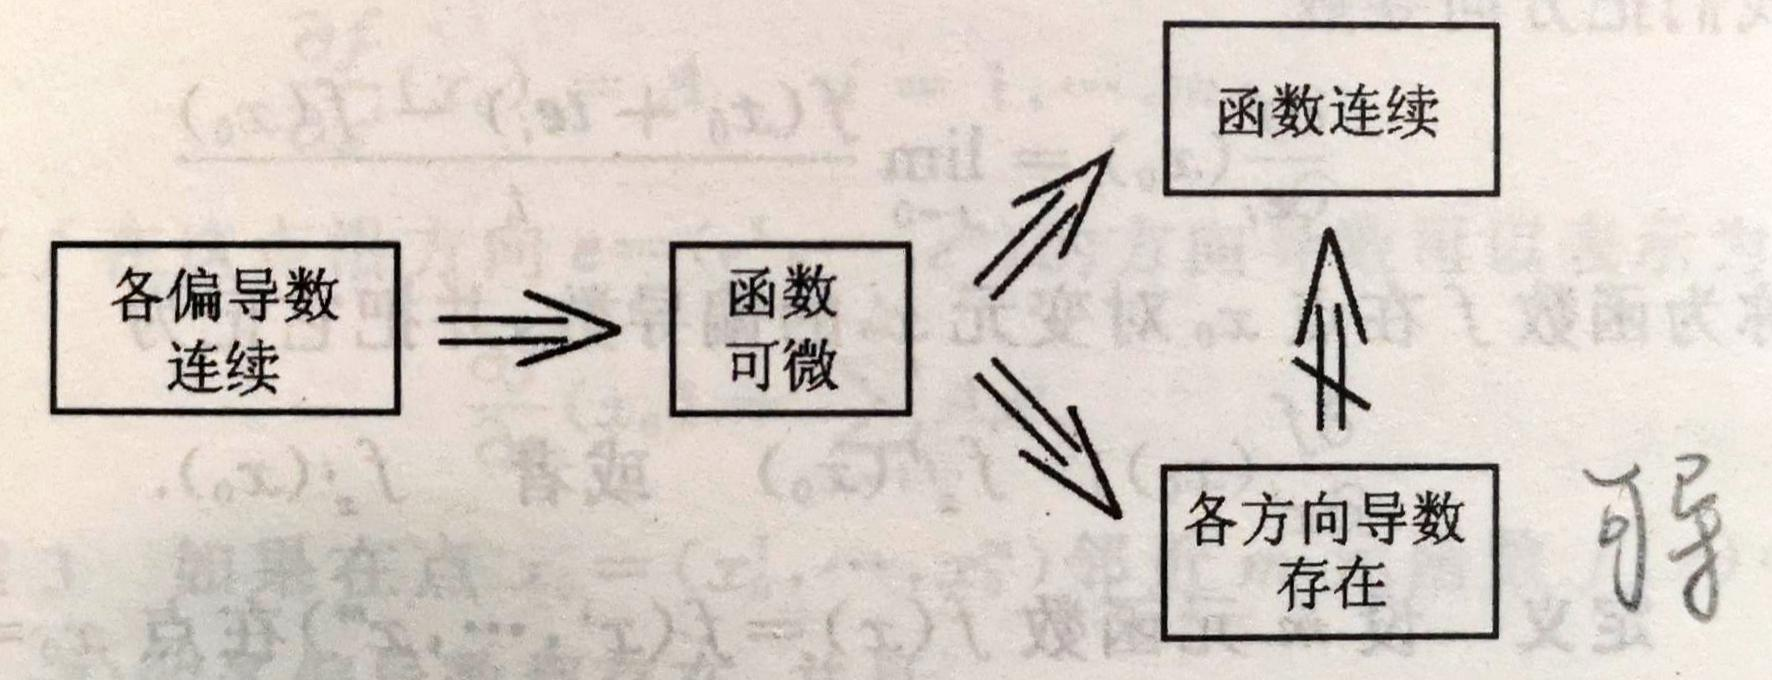
\includegraphics[width = 0.5\linewidth]{./images/differentiation.jpg}
    \caption{连续, 可导, 可微的关系}
\end{figure}

\subsection{多元函数的导数等价定义}
考虑一元函数的导数定义: \[ \dd {f}.{x} = \lim_{h \to 0} \dfrac{f(x + h) - f(x)}{h} \,.\]

若直接将一元变量替换向量, \[ \pp {f}.{\ve x} = \lim_{\ve h \to \ve 0} \dfrac{f(\ve x + \ve h) - f(\ve x)}{\ve h} \,,\]

显然, 没法除以一个向量, 尝试使用向量的模(范数):
\[ \pp {f}.{\ve x} = \lim_{\ve h \to \ve 0} \dfrac{f(\ve x + \ve h) - f(\ve x)}{\|\ve h\|} \,,\]

但这样也有问题, 考虑一维情况, 之前分子和分母的 $ h $ 可以取负数; 现在无论一维的 $ \ve h $ 取正还是负, 分母 $ \| \ve h \| $ 都是正. 这样会带来符号上的错误. 所以要采用其它定义方式.

\begin{definition}[\text{一元函数可微}]
    函数 $ f $ 可微, 当且仅当 \[ \lim_{h \to 0} \dfrac{f(a + h) - f(a) - mh }{h} = 0 \,,\] 此时 $ m $ 为函数的导数.
\end{definition}

如此改写定义之后, 无论分母加不加绝对值, 都不会影响可微的定义:
\[ \lim_{h \to 0} \dfrac{f(a + h) - f(a) - mh }{|h|} = 0 \]

也是正确的, 如果 $ h < 0 $, 不过是极限前加符号, $ +0 $ 和 $ -0 $ 没有区别, 故不影响判断:
\[ \lim_{h \to 0} \dfrac{f(a + h) - f(a) - mh }{-h} = - \lim_{h \to 0} \dfrac{f(a + h) - f(a) - mh }{h} = 0 \,.\]

这样就可以拓广到多元函数.

\begin{definition}[\text{多元函数可微}]
    函数 $ \ve f: U \subseteq \R^n \to \R^m $ 可微, 当且仅当存在一个线性映射 $ \ve L: \R^n \to \R^m $, 满足:\[ \lim_{\ve h \to \ve 0} \dfrac{\| \ve f(\ve x + \ve h) - \ve f(\ve x) - \ve L \ve h \|}{\|\ve h\|} = 0 \,.\] 如果 $ f $ 可微, 则函数各偏导存在, $ \ve L $ 由雅可比矩阵给出: \[ \ve L = D\ve f(\ve x) \,.\]
\end{definition}







\appendix
\newpage
\section{补充知识}
\subsection{扩展实数域}
若将 $ \pm \infty $ 作为 $ \R $ 的两个元素, 则能得到扩展实数域 $ \overline \R $. 我们可以规定无穷元素之间及其和其它有限元素的运算($ \infty = \pm \infty $), 如:
\[ +\infty = -(-\infty) \,,\]
\[ a \pm \infty = \pm\infty \,,\]
\[ a \cdot (+\infty) = 
    \begin{cases}
        + \infty & a \text{ 为正数} \\
        - \infty & a \text{ 为负数}
    \end{cases}\,,
\]
\[ +\infty + (+\infty) = +\infty \,,\]
\[ \pm\infty \cdot (\pm\infty) = +\infty  \,,\]
\[ \pm\infty \cdot (\mp\infty) = -\infty \,,\]
\[ \dfrac{a}{\pm\infty} = 0 \ (a \text{ 为正数})\,,\]
\[ \dfrac{a}{0^\pm} = \pm \infty \ (a \text{ 为正数})\,.\]

其中, $ 0^+ $ 表示从正向趋于 $ 0 $, $ 0^- $ 表示从负向趋于 $ 0 $.

而下面的式子没有统一的极限, 称为未定式, 如:
\[ +\infty - \infty \,,\] 
\[ 0 \cdot \infty \,,\]
\[ \infty^0 \text{ 和 } 1^\infty \text{ 和 } 0^0 \,,\]
\[ \dfrac{0}{0} \text{ 和 } \dfrac{\infty}{\infty} \,,\]

\subsection{函数空间}
设 $ I $ 是一个区间, $ C^0 (I) $ 表示所有 $ I $ 上连续的函数的集合. 所以如果有 $ f \in C^0 (I) $ 表示 $ f $ 在 $ I $ 上连续.

$ C^n (I) $ 表示所有 $ I $ 上 $ n $ 阶导数连续的函数集合. 如 $ f \in C^1 (a, b) $ 表示 $ f $ 在 $ (a, b) $ 上一阶导函数连续, 也就是函数在 $ (a, b) $ 上可导.

\newpage
\section{部分定理证明}
\begin{theorem}[\text{确界存在定理}] 
    非空有上/下界的数集必有上/下确界.
\end{theorem}

\begin{proof}
    任意一个实数 $ x \in \R $ 都可以写作小数形式 $ x = [x] + (x) $, 其中 $ [x] $ 为整数部分, $ (x) $ 为小数部分. $ x $ 可以逐位写出 $ x_0.x_1 x_2 \cdots $, 其中 $ x_i \ (i \geqslant 1) \in \{0, 1, 2, \dots, 9\} $. 约定下面两点:
    \begin{itemize}
        \item 若为有限小数, $ x_0.x_1 x_2 \cdots x_n $, 则第 $ n $ 位后面用 $ 0 $ 填充, 等价于 $ x_0.x_1 x_2 \cdots x_n 00 \cdots $
        \item $ x_0.x_1 x_2 \cdots x_n \cdots = x_0.x_1 x_2 \cdots (x_n - 1) 999 \cdots $
    \end{itemize}

    下面设集合 $ S $ 为有上界的非空数集, 证明 $ S $ 有上确界. 设 $ x = x_0.x_1 x_2 \cdots \in S $. 集合 $ S $ 可以描述为 $ S = \{ x_0 + 0.x_1 x_2 \cdots \mid x_0 = [x], 0.x_1 x_2 = (x) \cdots \} $.

    \paragraph{逐位筛选出最大数}
    先看整数位, 由于 $ S $ 有界, $ x_0 $ 必然不可能无限大, 选取使得 $ x $ 最大的整数位 $ x_0 $, 记为 $ \beta_0 $, 将这些数放入一个新集合中, 记作 $ S_0 = \{ x \in S \mid x \text{ 整数位最大} \} $. 也就是说 $ S_0 $ 中包含所有整数位为 $ \beta_0 $ 的数.

    接着筛选第一位小数, 将使得 $ S_0 $ 中的数最大的第一位小数筛选出来, 记作 $ \beta_1 $, 将第一位小数为 $ \beta_1 $ 的数放入一个新集合中, 记作 $ S_1 = \{ x \in S_0 \mid x \text{ 第一位小数为 } \beta_1 \} $. 也就是说 $ S_1 $ 中包含整数位为 $ \beta_0 $, 小数位为 $ \beta_1 $ 的数.

    重复上面的过程, 逐位筛选, 得到使得 $ S_{n - 1} $ 中的数最大的第 $ n $ 位小数位 $ \beta_n $. $ S_n = \{ x \in S_{n-1} \mid x \text{ 第 } n \text{ 位小数为} \beta_n \} $.

    用 $ \square $ 表示任意 0 到 9 的整数, $ S_0 $ 到 $ S_1 $ 中分别包含:

    $ S_0 : \beta_0.\square\square\square \cdots $

    $ S_1 : \beta_0.\beta_1 \square\square\cdots $

    $ S_2 : \beta_0.\beta_1\beta_2 \square \cdots $

    $ \vdots $

    $ S_n : \beta_0.\beta_1\beta_2 \cdots \beta_n \square\square \cdots $

    而这些集合形成了一个``区间套'': $ S_0 \supseteq S_1 \supseteq S_2 \supseteq \cdots \supseteq S_n $. 注意可以取等, 这很重要.

    \begin{figure}[H]
        \centering
        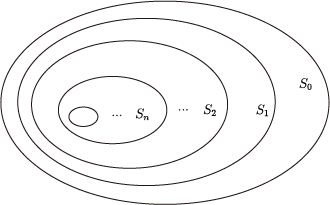
\includegraphics[width = 0.4\linewidth]{./images/nested.png}
    \end{figure}

    按照这一规则, 重复操作, 可以选出一个数 $ \beta = \beta_0. \beta_1 \beta_2 \cdots \beta_n \beta_{n + 1} \cdots $

    \paragraph{证明 $ \beta $ 是上界}
    要证明 $ \beta $ 是上界, 即证明 $ \forall x \in S $, $ x \leqslant \beta $. 由于 $ x $ 只有两种情况: 1.\, $ x $ 在每一个集合中, 即 $ \forall n \in \N $, $ x \in S_n $. 设想区间套是一叠纸片, 集合里的元素为一根针, 此时这根针 $ x $ 扎在这一叠纸片中, 能将所有纸片固定在墙上, 因为穿过了所有纸片  2.\, $ x $ 不在每一个集合中, 也即 $ \exists n_0 \in \N $, $ x \not\in S_{n_0} $. 这根针没有穿过所有纸片, 固定在墙上是有纸片会掉落. 所以可以讨论这两种情况:
    \begin{enumerate}
        \item $ \forall n \in \N $, $ x \in S_n $ \\
            $ x = \beta $
        \item $ \exists n_0 \in \N $, $ x \not\in S_{n_0} $ \\
            $ x = \beta_0.\beta_1 \beta_2 \cdots \beta_{n_0} x_{n_0 + 1} \cdots \leqslant \beta_0.\beta_1 \beta_2 \cdots \beta_{n_0} \beta_{n_0 + 1} \cdots = \beta $
    \end{enumerate}

    综上所述, 对于任意 $ x $ 要么等于 $ \beta $, 要么小于等于 $ \beta $, 所以 $ \beta $ 为上界.

    \paragraph{证明 $ \beta $ 是最小上界}
    即证明 $ \forall \epsilon > 0 $, $ \exists x \in S $, $ \beta - \epsilon < x $.

    取 $ n_0 \in \N $, 使其满足 $ \dfrac{1}{10^{n_0}} < \epsilon $. 

    考察 $ x \in S_{n_0} $, $ x = \beta_0.\beta_1 \beta_2 \cdots \beta_{n_0} x_{n_0 + 1} \cdots $, 
    
    $ \beta - \epsilon = \beta_0.\beta_1 \beta_2 \cdots (\beta_{n_0} - 1) \beta_{n_0 + 1} \cdots < x $.
\end{proof}

\begin{theorem}[\text{紧致集上的函数最值}]
    紧致集 $ C \subset \R^n $ 上的函数 $ f : C \to \R $ 连续. 则存在点 $ \ve a \in C $ 使得对 $ \forall \ve x \in C $ 都有 $ f(\ve a) \geqslant f(\ve x) $, 即最大值. 同理存在 $ \ve b \in C $ 使得 $ \forall \ve x \in C $ 都有 $ f(\ve b) \leqslant f(\ve x) $, 即最小值.
\end{theorem}

\begin{proof}
    
\end{proof}


\end{document}